\section{Paper II: Automatic sleep stage classification with deep residual networks in a mixed-cohort setting}\label{sec:paperii}
\sectionmark{Olesen, Jennum, Mignot, \& Sorensen, 2020 (\textit{submitted)}}



\subsection{Cohort descriptions}
To investigate and conclude on generalizability of any machine learning or sleep stage classification model, multiple heterogenous datasets must be used for training, validation and testing purposes.
In this work, we collected datasets from five different sources, each dataset containing a diverse collection of subjects presenting with multiple disease phenotypes.
Details of the separate cohorts are shown in Table 1 along with reported \textit{p}-values highlighting cohort differences.
Each cohort was split into a training, validation and testing subset in proportions of 87.5\%, 2.5\% and 10\%, respectively, using random sampling without replacement among unique subjects, so that no subject is shared between subsets.
With these percentages, we maximize the number of PSGs available for training, while still reserving enough PSGs for validation and testing.
Collecting all the separate subsets across cohorts forms a training, validation, and testing partition, containing the respective subsets from all five cohorts. 

\subsubsection{Institute of Systems and Robotics, University of Coimbra Sleep Cohort (ISRUC)}
This cohort contains 126 recordings from 118 unique subjects recorded at the Sleep Medicine Centre of the Hospital of Coimbra University, Portugal, in the period 2009–2013~\cite{Khalighi2016}.
The cohort comprises three subgroups: subgroup I contains 100 PSGs of subjects with diagnosed sleep disorders, generally sleep apnea; subgroup II contains 16 recordings of eight subjects most of which are also diagnosed with sleep apnea; and subgroup III contains recordings from 10 subjects with no diagnosed sleep disorders.
All PSGs were recorded with the same recording hardware and software and each was scored by two technicians for sleep stages and sleep events according to the AASM guidelines.
ISRUC-Sleep is a freely accessible resource and all data and PSG files can be located at \url{https://sleeptight.isr.uc.pt/ISRUC_Sleep/}.

\subsubsection{The MrOS Sleep Study (MrOS)}
The MrOS sleep study is part of the larger Osteoporotic Fractures in Men Study, which aims to understand the relationships between sleep disorders, fractures, and vascular diseases in community-dwelling men~\cite{Blank2005, Orwoll2005, Blackwell2011}. 
It consists of 2907 in-home PSG recordings with an additional 1026 follow-up PSG studies from subjects recruited from six different clinical centers in the USA.
Each recording was annotated by an expert technician according to Rechtschaffen and Kales (R\&K) criteria for sleep staging~\cite{Rechtschaffen1968}.
For compatibility with AASM guidelines, we combined stages labeled S3 and S4 into N3. All data were accessed from the National Sleep Research Resource (NSRR) repository~\cite{Dean2016, Zhang2018}.

\subsubsection{The Sleep Heart Health Study (SHHS)}
The SHHS is a large, multi-center study on cardiovascular outcomes related to sleep disorders with a specific focus on sleep-disordered breathing~\cite{Redline1998, Quan1997}.
The cohort consists of 6441 subjects above 40 years old recruited between 1995 and 1998 undergoing in-home PSG (SHHS Visit 1) with subsequent follow-up PSG between 2001 and 2003 in 3295 subjects (SHHS Visit 2).
PSG recordings were annotated for sleep stages by trained and certified technicians according to R\&K rules.
From the original cohort we extracted 5793 PSGs and annotations from Visit 1, and 2651 from Visit 2.
We aggregated S3 and S4 stages into N3 similar to MrOS.
All data were accessed from NSRR repository.

\subsubsection{Wisconsin Sleep Cohort (WSC)}
WSC is a population-based study of sleep-disordered breathing in government workers in Wisconsin, USA that was initiated in 1988~\cite{Young1993, Young2008}.
In this work, we used 2412 PSGs from 1091 unique subjects in the WSC sample scored by expert technicians according to R\&K rules with subsequent merging of S3 and S4 into N3.

\subsubsection{Stanford Sleep Cohort (SSC)}
PSGs from this cohort originate from patients referred for sleep disorders evaluation and recorded at the Stanford Sleep Clinic since 1999.
The specific sample used in this study represents a small subset ($n=772$) of the whole cohort, which was selected and described in detail in previous studies scored according to R\&K or AASM guidelines according to prevailing standard at the time of evaluation~\cite{Andlauer2013, Moore2014}. 


\subsection{Methods}
\subsubsection{Data pipeline}
Electrophysiological signals corresponding to the minimum acceptable montage for sleep staging available across all cohorts were extracted for each PSG.
These included a central EEG (either C3 or C4 referenced to the contra-lateral mastoid), left and right EOG referenced to the contra-lateral mastoid, and a single submentalis EMG.
The choice between C3 and C4 was determined based on the lowest total signal energy across the entire duration of the PSG to avoid excessive signal popping.
Other methods to determine appropriate channels include algorithms based on shortest Mahalanobis distance to an already determined reference distribution~\cite{Stephansen2018}, but was not investigated in this study.
All signals were resampled to $f_s = \SI{128}{\hertz}$ using a polyphase filtering procedure irrespective of original sampling frequency, and subsequently filtered using a zero-phase approach with \nth{4} order Butterworth IIR filters (0.5 to 35 Hz band pass for EEG and EOG; 10 Hz high pass for EMG) in accordance with AASM filter specifications~\cite{Berry2020}.
Each signal was normalized to zero mean and unit variance to accommodate differences in recording equipment and baselines, and to compress the dynamic range into something easily trainable for the neural network architecture.
We denote by $C$ the number of input signals supplied to the neural network, where in this case $C=4$.

\subsubsection{Machine learning problem}
We designate by $\mathcal{X} \in \real^{C \times T}$ the set of \SI{30}{\second} input data segments with $S$ input channels and segment length $T$, and the corresponding sleep stage classifications by $\mathcal{Y} = \lbrace y \in \real_{+}^{K} \mid \sum_i y_i = 1 \rbrace$, where $K = 5$ corresponds to the five sleep stages.
Thus, $y$ is a probability simplex, which maps to the ordered set $\mathcal{S} = \lbrace \wake, \nI, \nII, \nIII, \rem \rbrace$ by the argmax function such that $\argmax{y : \mathcal{Y} \to \mathcal{S}}$.
Furthermore, as we are potentially interested in classifying multiple sleep stages at once, we extend the problem of classifying a single sleep stage given $x \in \mathcal{X}$ to a sequence-to-sequence problem, in which we desire to learn a differentiable function representation $\Phi$, that maps a sequence of \SI{30}{\second} epochs $\mathbf{x} \in \real^{C \times \alpha T}$ to their corresponding label probabilities $\mathbf{y} \in \real^{K \times \alpha}$, where $\alpha$ is a parameter that controls the sequence length. 
For example, if $\alpha=8$, the sequence $\mathbf{x}$ contains \SI{4}{\minute} of successive PSG data described by 8 epochs of length \SI{30}{\second}.
Furthermore, we denote by $\llbracket a, b \rrbracket$ the set of integers from $a$ to $b$, i.e. $\llbracket a, b \rrbracket = \lbrace n \in \mathbb{N} \mid a \leq n \leq b \rbrace$, and by $\llbracket N \rrbracket$ the shorthand form of $\llbracket 1, N \rrbracket$.

\subsubsection{Network architecture}
\begin{figure}
    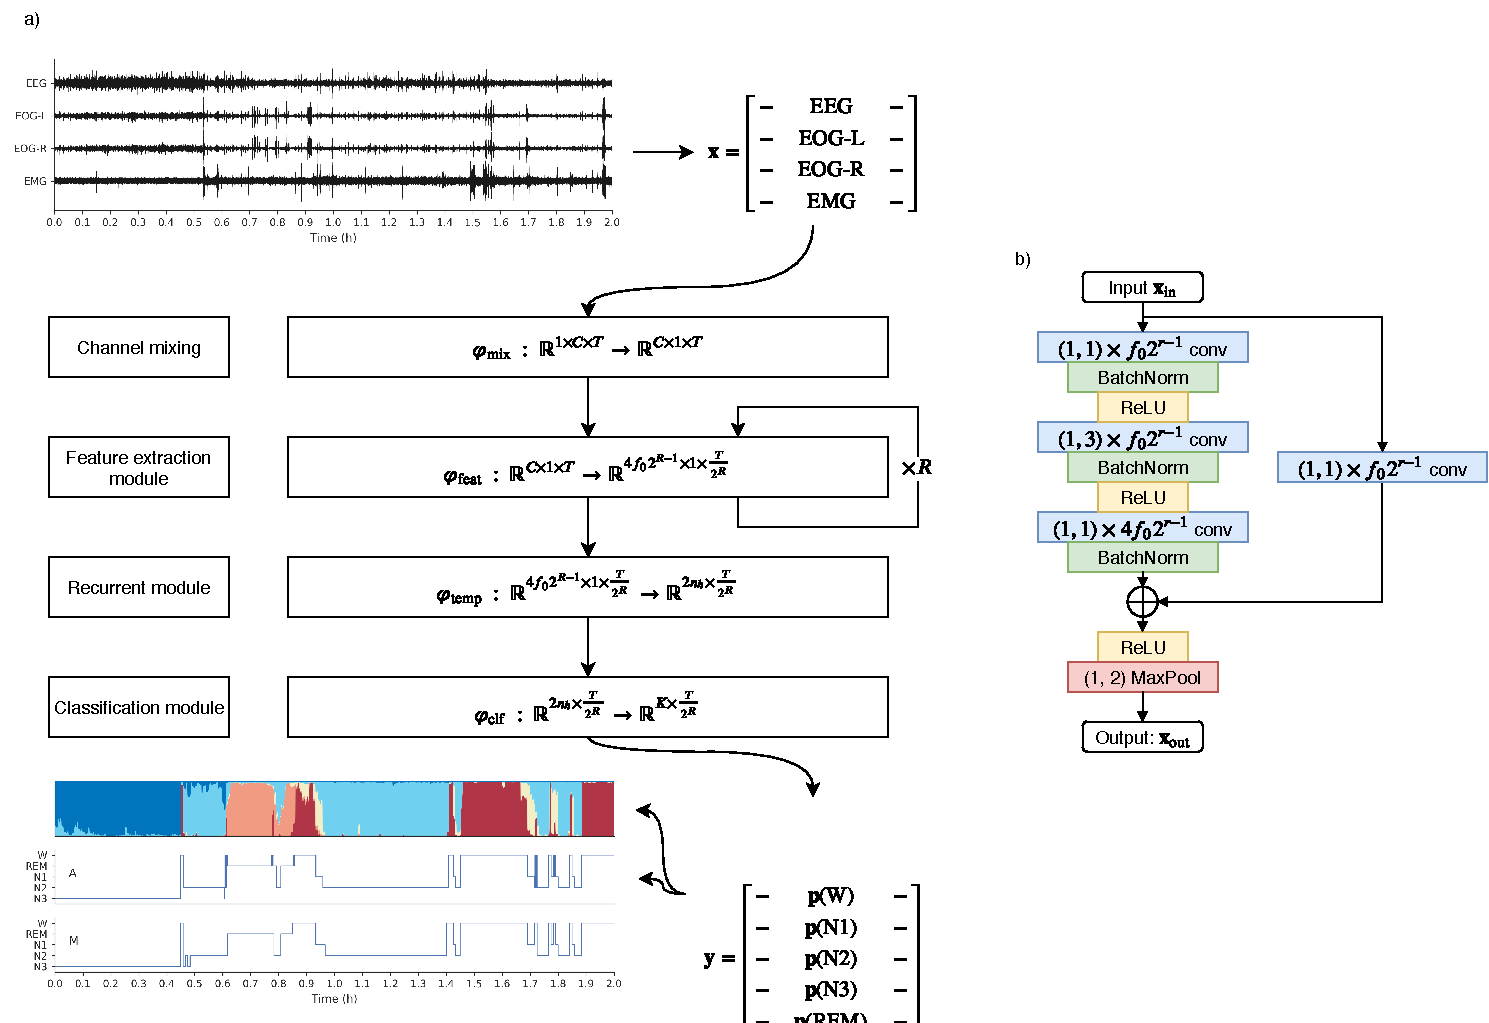
\includegraphics[width=\textwidth+\marginparwidth+\marginparsep]{figures/paper-ii/figure_01_a-b.pdf}
    \caption{Caption}
    \label{fig:paper-ii-figure1}
\end{figure}
As the representation of $\Phi$, we adapted and extended a previously published neural network architecture for automatic sleep stage classification, which was based on a variant of the ResNet-50 architecture commonly used for two-dimensional image classification tasks, but adapted and re-trained from scratch for the specific use-case of one-dimensional, time-dependent signals in the PSG~\cite{Olesen2018c}.
This network has the advantage that it does not require any manual feature engineering and extraction compared to previous state of the art sleep stage classification models~\cite{Stephansen2018}.
An overview of the proposed network architecture is provided graphically in Figure 1 and Table 2.
Briefly, the architecture consists of four modules:
\begin{enumerate}
    \item an initial mixing module 
    \begin{equation}
        \varphi_{\mathrm{mix}} : \real^{1 \times C \times T} \to \real^{C \times 1 \times T},
    \end{equation}%$\varphi_{\mathrm{mix}} : \real^{1 \times C \times T} \to \real^{C \times 1 \times T} $,
	\item a feature extraction module
	\begin{equation}
	    \varphi_{\mathrm{feat}} : \real^{C \times 1 \times T} \to \real^{f_0 2^{R+1} \times 1 \times T/2^R},
	\end{equation}
	\item a temporal processing module
	\begin{equation}
	    \varphi_{\mathrm{temp}}     : \real^{f_0 2^{R+1} \times 1 \times T/2^R} \to \real^{2n_h \times T/2^R}, \, \text{and}
	\end{equation} %$\varphi_{\mathrm{temp}}     : \real^{f_0 2^{R+1} \times 1 \times T/2^R} \to \real^{2n_h \times T/2^R} $, and
	\item a classification module
	\begin{equation}
	    \varphi_{\mathrm{clf}} : \real^{2n_h \times T/2^R} \to \real^{K \times T/2^R}.
	\end{equation}%$\varphi_{\mathrm{clf}} : \real^{2n_h \times T/2^R} \to \real^{K \times T/2^R}$.
\end{enumerate}
Thus, we obtain a differentiable representation of the function  $\Phi$ as
\begin{align}
\begin{split}
    &\Phi : \real^{C \times K} \to \real^{K \times T/2^R} \\
    &\Phi\left(\mathbf{x}\right) = \varphi_{\mathrm{clf}} \left( \varphi_{\mathrm{temp}} \left( \varphi_{\mathrm{feat}} \left( \varphi_{\mathrm{mix}} \left( \mathbf{x} \right) \right) \right) \right).
\end{split}
\end{align}
The output of this function is the matrix $\mathbf{y} \in \real^{K \times T/2^R}$ containing sleep stage probabilities in the sequence of PSG data evaluated every second.

\paragraph{Mixing module}
The raw input data is input to this module, which encourages non-linear channel mixing similar to what has been proposed in recent literature~\cite{Chambon2018c, Chambon2018b, Chambon2019, Olesen2019}.
The module is realized using a single 2D convolutional operation outputting $C$ feature maps computed using single-strided $(C \times 1)$ kernels followed by rectified linear unit (ReLU) activations.

\paragraph{Feature extraction (residual network) module}
This is comprised of a succession of $R$ residual blocks (see Figure 1)\todo{fix}, which are responsible for the bulk feature extraction from the channel-mixed data.
Each residual block is realized using bottlenecks of first a $1\times 1$ convolution to reduce the number of feature maps, then a $1\times 3$ convolution, and lastly a $1 \times 1$ convolution to finally increase the number of feature maps. 
Each convolution operation is followed by a batch normalization~\cite{Ioffe2015} and ReLU activation except after the last convolutional layer, where shortcut projections are added before the activation~\cite{He2016b}.
This type of block structure enables the design and training of very deep networks without the risk of vanishing gradients due to the projection shortcuts~\cite{He2016}.

\paragraph{Temporal processing module}
This module is realized by a bidirectional gated recurrent unit (GRU)~\cite{Cho}45 in order to accommodate temporal dependencies in the PSG.
The GRU runs through the temporal dimension of the output from $\varphi_{\mathrm{feat}}$ of $T/2^R$ time steps each containing $f_0 2^{R+1}$ feature maps and outputs $n_h$ new features in each direction for each time step.
By running both forward and backward, we can accommodate that technicians base their scoring on looking backwards as well as ahead in time in each time segment (typically 30 s).

\paragraph{Classification module}
The final module in the architecture performs actual classification based on the forward and backward features for each time step outputted from $\varphi_{\mathrm{temp}}$.
It is realized by a single convolutional operation with a subsequent softmax activation to compute a probability distribution over the $K$ sleep stage classes, such that the probability of sleep stage $i$ at time step $n$ is given by $y_i^{(n)} = \frac{\exp{a_i}}{\sum_k{\exp{a_k}}}$)), where $a_i \in \mathbf{a}$ is the activation of the last layer in the network and $k=\llbracket K \rrbracket$.


\subsubsection{Loss function specification}
The network was trained end-to-end with respect to a loss function, that takes the output probabilities from the network $y = \Phi\left( \mathbf{x} \right)$ and calculates the loss as
\begin{align}
\begin{split}\label{eq:loss-paperII}
    \mathcal{L}\left( \mathbf{y} \right) &= - \sum_{n=1}^{30/\tau}\sum_{k=1}^{K} t_k^{(n)}\log{\left( \tilde{y}^{(n)}_k \right)}, \\
    \tilde{y}^{(n)}_k &= \frac{1}{\tau} \sum_{i=\tau \left( j - 1 \right) + 1}^{\tau n} y_k^{(i)},
\end{split}
\end{align}
which is the cross-entropy between successive time-averaged classifications parameterized by the number of successive one-second predictions $\tau$, and the ground truth labels $t$ broadcasted to $\frac{30}{\tau}$ labels per \SI{30}{\second} segment.
This way, we can acquire predictions every second, that can be combined in time at intervals given by $\tau$.

\subsubsection{Experimental setups}
We set up three different experiments in this study.
\begin{enumerate}
    \item We wished to investigate the effect of increasing the complexity of the recurrent module by varying the number of units $n_h$ in the module $\varphi_{\mathrm{temp}}$ in the space $n_h=2^k, k \in \llbracket 6, 11 \rrbracket$.
    We hypothesize that there exists a sweet-spot in the number of hidden units that balances computational complexity with classification performance, i.e. classifying a sequence of sleep stage labels given a corresponding sequence of outputs from $\varphi_{\mathrm{feat}}$.
    The results of this experiment were furthermore used to determine parameters for models in subsequent experiments.
    \item Since we have several cohorts at our disposition of both clinical and research origin, we can investigate the compatibility and inherent generalizability of the different cohorts in two ways: 1) we set aside a single cohort for testing, while we train the models on the remaining four (leave-one-cohort-out, LOCO training); and 2) we train on a single cohort, while we set aside the remaining four for testing (leave-one-cohort-in, LOCI training).
    \item Generalizability can also be investigated in another way, which can answer the question of how many data sources is necessary.
    We trained models with all possible 2-, 3-, and 4-combinations of cohorts, i.e. one run trained on ISRUC and MrOS training data, another run with ISRUC and SHHS train data, a third with ISRUC and SSC, etc., with all runs subjected to subsequent evaluation on the test partition. 
    \item Previous studies have already investigated the performance of automatic sleep staging algorithms using shallow machine learning models.
    At the time of writing however, none have investigated the effect of available training data for deep learning models at this magnitude (up to tens of thousands).
    We therefore trained models on 0.25\%, 0.5\%, 1\%, 5\%, 10\%, 25\%, 50\%, 75\% and 100\% of the data available for training.
    Specifically, some of these fractions of the total number of PSGs correspond roughly to the number of PSGs in the training partitions in each cohort, allowing for direct comparisons between training a model with mixed- and single-cohort training data.
\end{enumerate}

Common for all experiments were the default parameter values $C=4$, $f_s=\SI{128}{\hertz}$, $T=\tau f_s$, $K=5$, $R=7$, and $f_0=4$ for the number of input channels, sampling frequency, the sequence length, the number of sleep stages, the number of consecutive residual blocks, and the base filter kernel size, respectively.
All models were trained for 50 epochs (passes through the training partition) and the model with the highest Cohen’s kappa value on the validation partition was subsequently selected for testing.
All models were trained end-to-end with backpropagation using the Adam optimizer~\cite{Kingma2015} with a learning rate of $10^{-4}$, $\beta_1=0.9$, and $\beta_2=0.999$ to minimize the loss function specified by \cref{eq:loss-paperII}. 
All network weights and bias terms were initialized using the uniform Glorot initialization scheme~\cite{Glorot2010}. 

\subsubsection{Performance metrics and model evaluation}
For each experiment we evaluated model performance using the overall accuracy (Acc) and \cohen in order to take account the possibility of chance agreement between the model and the gold standard.
Given a confusion matrix $\mathbf{C}$ with element $c_{ij}$ being the number of epochs belonging to sleep stage $i$ but classified to be in sleep stage $j$, we define the overall accuracy for a given model as
\begin{equation}
    \text{Acc} = \frac{\sum_{i=j}c_{ij}}{\sum_{i,j}c_{ij}},
\end{equation}
\ie the sum of the trace of $\mathbf{C}$ divided by the total count.
The \cohen metric is defined as
\begin{equation}
    \kappa = \frac{p_o - p_e}{1 - p_e},
\end{equation}
where $p_o = \text{Acc}$ is the observed agreement (\ie accuracy) and $p_e$ is the expected chance agreement, which can be reformulated in terms of the outer product between the row and column sums (class-specific recall and precision) of $\mathbf{C}$.


\subsection{Results}

\subsubsection{Temporal context impact on model performance}
\begin{figure}
    \centering
    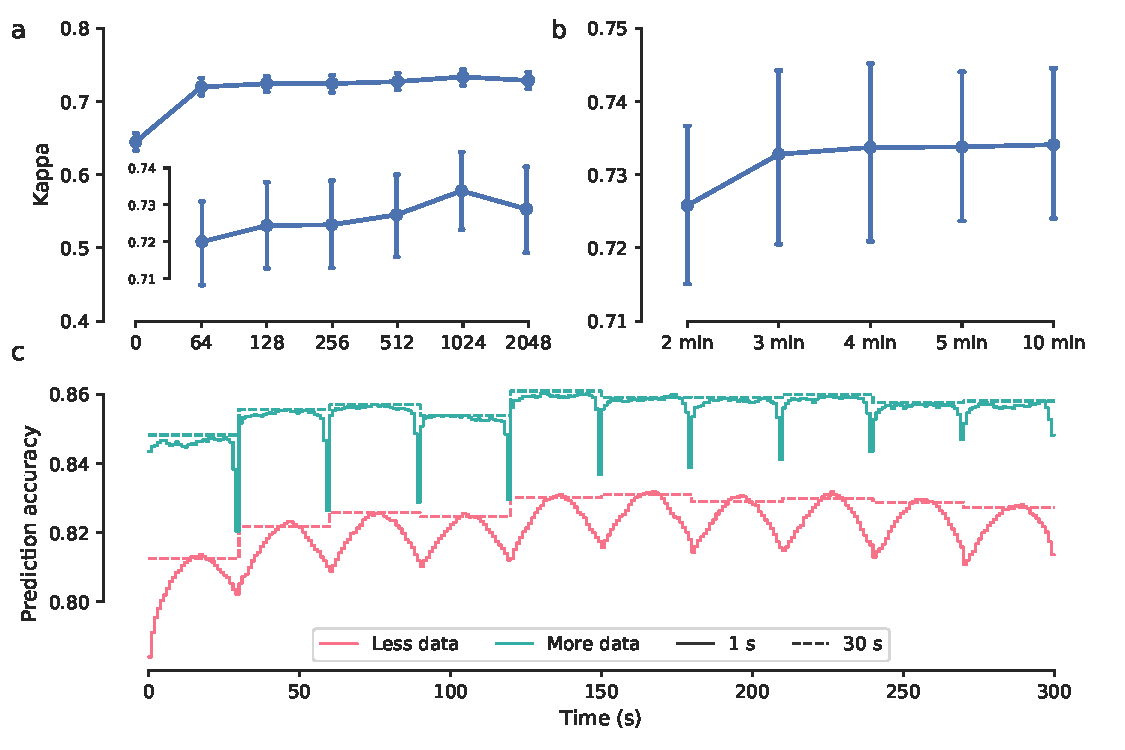
\includegraphics[width=\columnwidth]{figures/paper-ii/figure_02_a-c.pdf}
    \caption[MASSCv2 temporal context]{Caption}
    \label{fig:paper-ii-figure2}
\end{figure}
In~\cref{fig:paper-ii-figure2} we show how the model performance depends on the temporal context and complexity of the temporal processing module, when evaluating the model on the validation partition.
Results are further detailed in Table S1\todo{supplementary tables???}.
Specifically, we observe a drastic change in \cohen just by introducing a simple recurrent unit into the network as shown in~\cref{fig:paper-ii-figure2}a, where \cohen increases from \ci{0.645}{0.126}{0.633}{0.657} at $n_h=0$ to \ci{0.720}{0.120}{0.709}{0.731} at $n_h=64$. 
We did not observe any major changes when increasing the number of hidden units beyond $n_h=64$, although we did see a maximum \cohen of \ci{0.734}{0.111}{0.723}{0.744} at $n_h=1024$, which is shown in the inset in~\cref{fig:paper-ii-figure2}a. 
We observed a general increase in \cohen when classifying longer sequences than \SI{2}{\minute} (\ci{0.726}{0.114}{0.715}{0.737}), but did not see any major differences when classifying over more than \SI{3}{\minute} sequences (\ci{0.733}{0.123}{0.721}{0.7444}).
Subsequent models were fixed with $n_h=1024$ corresponding to a sequence length of \SI{5}{\minute}.

\subsubsection{Model classifications converge to 30 s predictions given sufficient training data}
Furthermore, we analyzed the classification performance of the model given a specific sequence length by looking at the average prediction accuracy across all \SI{5}{\minute} sequences in all subject PSGs in the test partition, similar to what~\citeauthor{Brink-Kjaer2019} has shown previously~\cite{Brink-Kjaer2019}.
In~\cref{fig:paper-ii-figure2}c, we show how the average classification accuracy in a \SI{5}{\minute} sequence both depends on the amount of data and the frequency of evaluating the model output, \ie every \SI{1}{\second} or across \SI{30}{\second}.
The average classification accuracy was found to be slightly lower in the beginning of each \SI{5}{\minute} sequence, both when training a model with less (500 training subjects) and more (\SI{75}{\percent} of total training subjects).
Interestingly, when training with less data, we also observed a lower accuracy in the beginning and end of each \SI{30}{\second} segment relative to the accuracy in the middle section, which was not the case when training with more data.

\subsubsection{Choice of cohort impacts classification performance on test set}
\begin{figure}
    \centering
    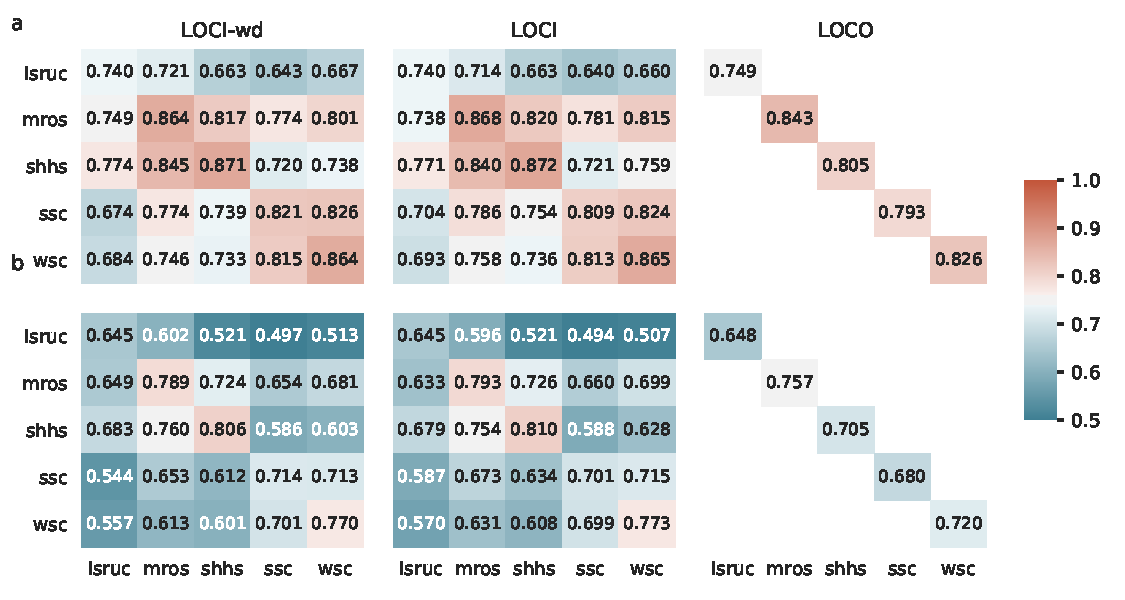
\includegraphics[width=\columnwidth]{figures/paper-ii/figure_03_a-b.pdf}
    \caption[MASSCv2 LOCI and LOCO performance]{Caption}
    \label{fig:paper-ii-figure3}
\end{figure}
In~\cref{fig:paper-ii-figure3} we show how training on different cohorts yield differing results in subsequent testing performance, here expressed in heatmaps as both overall accuracy (\cref{fig:paper-ii-figure3}a), and \cohen (\cref{fig:paper-ii-figure3}b) averaged across all $N=1584$ subject PSGs in the test partition.
The first two columns show the performance on the cohort on the \textit{x}-axis, when training on the specific cohort on the \textit{y}-axis.
Since the training subset in ISRUC is small compared to the other cohorts, we trained the models in the left-most column with weight decay of $10^{-4}$ to compensate for the risk of overfitting, however, by comparing the left and middle columns, we did not observe any specific gain in classification performance by doing so.
The right-most column shows the test performance for each cohort, when excluding that cohort from training.
We observe a significant spread in classification accuracy across the different cohorts with prediction on ISRUC being poorest, while prediction on MrOS data being best.
Further details can be found in Table S2\todo{Supp. tables?}.

\subsubsection{More data is good, diverse data is better}
\begin{figure}
    \centering
    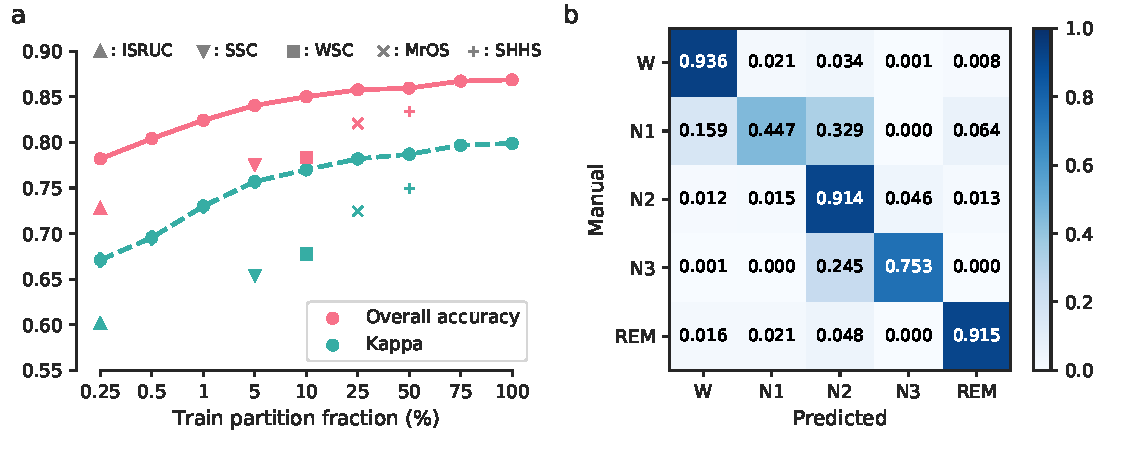
\includegraphics[width=\columnwidth]{figures/paper-ii/figure_04_a-b.pdf}
    \caption{Caption}
    \label{fig:paper-ii-figure4}
\end{figure}
We observed a general increase in classification performance both in terms of overall accuracy and \cohen, when including more data in the model training phase in both the mixed- and single-cohort setting (\cref{fig:paper-ii-figure4}a, Table S3\todo{Suppl. table}).
Classification performance was consistently lower in the single-cohort setting compared to the corresponding mixed-cohort setting. 
Interestingly, we found that training a model with just \SI{0.25}{\percent} of mixed-cohort training data still achieved an acceptable accuracy comparable to training a model with only SHHS data, while using all available training data increased that performance by almost 10 percentage points.
Furthermore, we observed that the model trained with \SI{100}{\percent} of the training partition reached a state-of-the-art level of performance with an overall accuracy of \ci{0.869}{0.064}{0.865}{0.872} and \cohen of \ci{0.799}{0.098}{0.794}{0.804} (see Table S3\todo{Suppl. table}).
The model furthermore performs well with respect to classifying individual sleep stages as shown in the confusion matrix in~\cref{fig:paper-ii-figure4}b.
However, the model still has difficulties classifying and distinguishing between certain sleep stages, especially between N2, N1, and N3; and W, N2, and N1.

\subsubsection{Increasing the number of data sources improves classification performance}
\begin{figure}
    \centering
    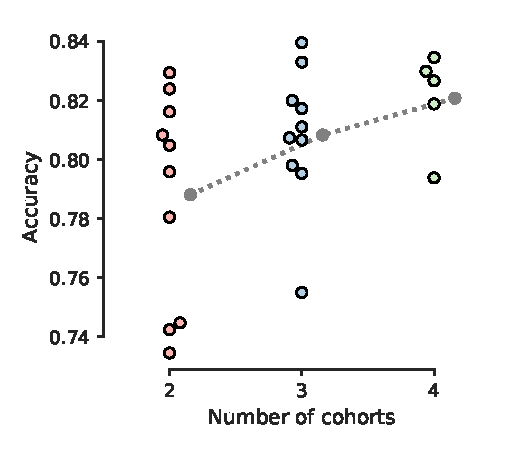
\includegraphics[width=0.75\columnwidth]{figures/paper-ii/figure_05.pdf}
    \caption{Caption}
    \label{fig:paper-ii-figure5}
\end{figure}
On average, we saw an increase in overall accuracy, when increasing the number of cohorts from 2 to 4 using 500 PSGs in each configuration, see~\cref{fig:paper-ii-figure5} and Table S4\todo{Suppl. table}.
Specifically, we found that the average overall accuracy increased from \ci{0.788}{0.102}{0.787}{0.790} in the 2-cohort configuration to \ci{0.808}{0.092}{0.807}{0.810} and \ci{0.821}{0.085}{0.819}{0.823} in the 3- and 4-cohort configurations, respectively.

\subsection{Discussion}
In this work, we present an end-to-end deep learning-based model for fully automatic micro- and macro-sleep stage classification. 
Using all of the available data sources for training our model, we reached an overall accuracy on test partition of \ci{0.869}{0.064}{0.865}{0.872}, and a \cohen of \ci{0.799}{0.098}{0.794}{0.804}, which is in the very high end of the substantial agreement category for observer agreement51.
We found that individual cohorts exhibit major differences in overall accuracy and \cohen when subjected to both training and testing conditions and specifically, we found that average performance on the test partition in the LOCI configurations varied significantly from \ci{0.676}{0.124}{0.670}{0.682} when training on ISRUC, to \ci{0.837}{0.084}{0.833}{0.841} when training on SHHS.
Each individual cohort also showed large deviations in predictive performance when tested on the other cohorts.
For example, when conditioned on SHHS data, the lowest average accuracy was 0.721 on SSC test data compared to the highest at 0.872 on SHHS test data, while conditioning on SSC training data, the lowest average accuracy was 0.704 on ISRUC test data compared to 0.824 on WSC test data.
Classification performance was generally higher on the test set when using the LOCO configuration, except for SHHS (higher in LOCI) and SSC (no difference).
We also found that having data from multiple sources always resulted in better-performing models compared to training on single cohorts.
Increasing the number of data sources increased classification performance, although this was non-significant.
In the design of the model, we observed that model performance was enhanced by the addition of the recurrent module (bGRU), a phenomenon likely reflecting the fact that sleep stage scoring at a specific time in one subject can be influenced by signal content (frequency, amplitude, presence of micro-events) at later time steps.
However, the complexity of the module given by the number of hidden units did not affect performance.
In all our experiments, we also evaluated the performance of the model every 1 s compared to the performance evaluated every 30 s and found them to be similar, which indicates the model is stable in classification in periods corresponding to an epoch of data.

Only a handful of studies have previously reported results when using multiple cohorts~\cite{Stephansen2018, Biswal2018a, Patanaik2018}.
Some authors have reported a drop from 81.9\% to 77.7\% when training on the Massachusetts General Hospital cohort (MGH) and testing on MGH and SHHS, respectively~\cite{Biswal2018a}, while others have shown significant drops from 89.8\% to 81.4\% and 72.1\% on two separate hold-out sets from Singapore and USA~\cite{Patanaik2018}.
We also observed similar trends in our LOCI and LOCO experiments, where excluding the training subset of a cohort from the training partition resulted in a significant drop in performance on the respective test subset from that cohort.
A benefit of our LOCI and LOCO experiments is the possibility for direct benchmarking against previous publications using specific cohorts in their experiments.
For example, we obtain an accuracy of 0.805 in the LOCO-SHHS training-testing case compared to 0.777 previously reported by~\citeauthor{Biswal2018a}~\cite{Biswal2018a}, both of which reflect classification performance when SHHS had not been used for training; and an accuracy of 0.865 in the LOCI-WSC case compared to 0.841 reported by \citeauthor{Olesen2018c}~\cite{Olesen2018c}, where both have been using a subset of WSC for training the model. 
Interestingly, we obtained the same level of performance on the SHHS data in our LOCI experiment as reported by \citeauthor{Sors2018} (87\% accuracy, 81\% \cohen) even though they only used single-EEG for their experiments~\cite{Sors2018}.
Other works that have investigated single- vs. multi-channel models for automatic sleep stage classification have found that models generally benefit from having more channels available for training~\cite{Chambon2018c, Biswal2018a, Phan2019a}.
It may be that some cohorts share different characteristics that makes them more suitable for single- or multi-channel models, but this is speculative and would need to be verified in subsequent studies.

We only optimized our network architecture with respect to the temporal processing module and therefore cannot assess what impact different design choices for the other modules would have had on final performance.
For example, the EMG signal has different statistical properties and spectral content, and separate, parallel architectures for EMG and EEG/EOG feature extraction may be warranted, as proposed by others~\cite{Chambon2018c, Stephansen2018}.
Other studies have however shown equal performance in large cohorts using a similar channel mixing approach as proposed here~\cite{Olesen2018c}.
Another limitation is found in our training runs, as we did not consider balancing our data with respect to the proportion of sleep stages, which may or may not have had impact on overall performance.
It is well established that there is significant variation in scoring and validation of N1/REM and N2/N3~\cite{Younes2016, Younes2018, Norman2000}, which challenges the training for any classification algorithm.
Some researchers have experimented balancing the cost of misclassifying sleep stages by weighting them by their inverse frequency of occurrence and found no significant improvement~\cite{Olesen2018c, Sors2018}, while others have experimented with balancing the sleep stage frequencies in each batch of data input to the neural network model~\cite{Chambon2018c}, but more rigorous research in resampling or over/under-sampling techniques is warranted in this regard.
We ultimately decided against experimenting with balancing our sleep stages in each batch, as we prioritized flexibility with regards to the length of input sequences fed to the network.
All our models ran through at least 50 epochs of training (passes through the training partition), which might have induced a bias in the configurations with larger cohorts.
For example, one pass through the training partition in the LOCI-ISRUC case corresponds to much less data than one pass through the LOCI-SHHS case.
However, since we selected the best performing model based on \cohen across all 50 epochs, we have allowed for more effective training in cases with less available training data.
We observed that models using less data in the training partition generally had to run for longer time (\ie more epochs) before converging.

In future studies on automatic sleep stage classification algorithms, we strongly recommend researchers to test and report results on not just hold-out test partitions, but also on cohorts completely unseen by the model both during training and testing/validation.
Our experiments indicate that even though good performance can be achieved on hold-out data using a single cohort, this does not necessarily translate into good generalization performance.
Such approach requires availability of many publicly available, high-quality, well-documented databases with easily accessible PSG data, associated annotations and related patient information.
In this regard, websites such as the NSRR, which contains several large databases with clinical data as well as PSG and annotation data in a standardized format~\cite{Dean2016,Zhang2018}, are an invaluable resource for researchers. 
We also propose that the sleep science community establishes a common reference dataset on which researchers in machine learning can benchmark their models, similar to what the computer vision and general machine learning community has done with the ImageNet Large Scale Visual Recognition Challenge (ILSVRC)~\cite{Russakovsky2015}, an annual competition in which researchers submit their models to test in various competitions.

In summary, we have developed an automatic sleep stage classification algorithm based on deep learning, that can accurately classify sleep stages at a flexible resolution with a state-of-the-art classification performance of 87\% accuracy on a test set of 1584 PSGs.
We trained and tested our model using five cohorts with varying numbers of PSGs covering multiple phenotypes with specific focus on how well cohorts can generalize to each other.
We found that different cohorts generalize very differently both in intra- and inter-cohort settings (LOCI vs. LOCO experiments).
Furthermore, we also found that having more data sources significantly improve classification performance and generalizability to the extent that even just a small number of training PSGs can reach high classification performance by including many different sources.
To our knowledge, this is one of the largest, if not the largest, study on automatic sleep stage classification in terms of PSG volume, diversity, and performance.
